\section{Fundamental building blocks}
% -----------------------------------------------------------------------------------
\subsection{Feed-forward NNs, Convolutional NNs, Residual NNs}
\begin{frame}{Different types of neural networks}
\begin{itemize}
\item There are \emphbf{different types of neural networks}, which are designed for different problems/sub-problems.
\item For those of you attending the Machine Learning lecture:\\
you have seen/will learn these models.
\item In this course: overview/reminder with \emphbf{example PyTorch code}.
\item[-] Opportunity to make sure you understand: input/output shapes, model parameters, ... how models work!
\item Outline:
\begin{itemize}
\item (Feed-forward neural networks): Exercise 4
\item Convolutional neural networks
\item Recurrent neural networks (RNNs), and long short-term memory (LSTM)
\item Neural attention, self-attention, and Transformers.
\end{itemize}
\end{itemize}
The assignments will cover concrete applications.
\end{frame}

\begin{frame}{Feed-forward neural networks}
We have already seen \emphbf{feed-forward neural networks} in the previous chapter:
\begin{itemize}
\item It's the basic model/layer to map/transform vectors.
\item It is also referred to as \textbf{multi-layer perceptron (MLP)}.\\
Even when it only has one hidden layer.
\item The main transformation is also referred to as a \textbf{fully connected} layer\\
(in contrast e.g. to a convolutional layer).
\item Terminology: \textit{feed-forward neural network} is a generic term for all neural networks which are \textbf{not recurrent}.
\end{itemize}
\end{frame}

\begin{frame}{Convolutional neural networks}
Typical shorthands: Convolutional nets, ConvNets, CNN.\\
\vsp
Typical convNets consist of a \textbf{stack} of:
\begin{itemize}
\item \emphbf{Convolutional layers}
\item \emphbf{Pooling layers} (e.g. max-pooling)
\item Fully connected layers
\end{itemize}
% Note, lecture by Sander Dieleman (Deepmind) at UCL, London:
% \link{https://www.youtube.com/watch?v=shVKhOmT0HE&feature=youtu.be}
\end{frame}

\begin{frame}{Convolutional layers, motivation}
\begin{itemize}
\item Remember what we did in the previous chapter?\\ For image classification using an MLP, we \textbf{reshaped input images to vectors},
and applied a linear transformation to them.
\vsp
\item Does this make sense? You might answer:
\begin{itemize}
\item Yes. We do not care, just plug-in input and output vectors to the model, and it learns the relationship. It's deep learning!
\item No. We should exploit properties of images to \textit{facilitate the learning problem} (jargon: we introduce an \textit{inductive bias} to the model architecture)
% pixels in images which could belong to a same entity in the image (locality), and also we need some translation invariance.
\end{itemize}
Which one sounds more reasonable? at this stage both?
\vsp
\pause
\item Original motivation: recognizing patterns in an image independent of its position.
\begin{itemize}
\item Locality (pixels which are close, likely belong to the same pattern): local connection.
\item Translation invariance.
\end{itemize}
\end{itemize}
\end{frame}

\begin{frame}{Convolutional layers, illustration}
\begin{minipage}{0.2\linewidth}
  \begin{center}
    \includegraphics[height=0.35\textheight]{figures/image-tree.png}
  \end{center}
Input image.
\end{minipage}
\hspace{2mm}
\begin{minipage}{0.35\linewidth}
  \begin{center}
    \includegraphics[height=0.35\textheight]{figures/fc-net.png}
  \end{center}
Fully connected layer.
\end{minipage}
\hspace{1mm}
\begin{minipage}{0.35\linewidth}
  \begin{center}
    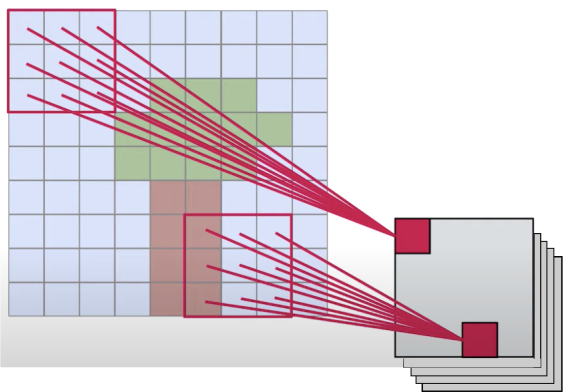
\includegraphics[height=0.4\textheight]{figures/convnet_v2.pdf}
  \end{center}
Convolutional layer.
\end{minipage}
\vfill
\scriptsize{Figures adapted from \citem{dieleman2020}.}\\
\vsp
\vsp
\normalsize{Check out more animated illustrations:}
\begin{itemize}
\item \link{https://github.com/vdumoulin/conv_arithmetic}\\
\item \link{https://cs231n.github.io/convolutional-networks/}
\end{itemize}
Also: lecture by Sander Dieleman (Deepmind) at UCL, London:
\link{https://www.youtube.com/watch?v=shVKhOmT0HE&feature=youtu.be}

\end{frame}

\begin{frame}{Convolutional layers, operation}
Description for 2D case. 2D convolutional layer:
\vsp
\begin{itemize}
\item \textbf{input}: image $x$ with shape ($C$, $H$, $W$) (let's omit batch for now)
\item  \textbf{output}: also image $y$ with shape ($C'$, $H'$, $W'$), \textit{feature map}
\item \textbf{model parameters}: weights and biases!
\begin{itemize}
\item Weights in a convnet consist of weights for \textit{kernels}.
\item Each convolutional layer contains $C'$ kernels ($C'$ = number of output channels).
\item Each kernel corresponds to weights of size ($C$, $d_{1}$, $d_{2}$). Here let's assume squared kernels $d=d_1=d_2$. They are small "image templates".
\item bias $b \in \mathbb{R}^{C'}$ 
\end{itemize}
\end{itemize}
\vsp
\vsp
\pause
 Given \textbf{input} $x \in \mathbb{R}^{C \times H \times W}$, for each each output channel $ 1 \leq k \leq C'$, \textbf{output} $y_{k, i, j}$ ($ 1 \leq i \leq H'$, and $ 1 \leq j \leq W'$) is computed using the corresponding \textbf{kernel} $f^{(k)}$ of size $d$ (i.e.\, $f^{(k)} \in \mathbb{R}^{C \times d \times d}$):
\[
y_{k, i, j} =  \sigma\left(b_{k} + \sum_{c=1}^{C} \sum_{i'=i}^{i+d-1} \sum_{j'=j}^{j+d-1} f^{(k)}_{c, i'-i+1, j'-j+1} \times x_{c, i', j'}\right)
\]
\end{frame}

\begin{frame}{Convolutional layers, operation (cont'd)}
% Given \textbf{input} $x \in \mathbb{R}^{C \times H \times W}$, for each each output channel $ 1 \leq k \leq C'$, \textbf{output} $y_{k, i, j}$ ($ 1 \leq i \leq H'$, and $ 1 \leq j \leq W'$) is computed using the corresponding \textbf{kernel} $f^{(k)}$ of size $K$:
%\[
%y_{k, i, j} =  \sigma\left(b_{i,j} + \sum_{c=1}^{C} \sum_{i'=i}^{i+K-1} \sum_{j'=j}^{j+K-1} f^{(k)}_{c, i'-i+1, j'-j+1} \times x_{c, i', j'} \right)
%\]
\begin{itemize}
\item Indices make it look complicated, but it is not!\\
 We are sliding each kernel on the input image.\\
See e.g. \link{https://github.com/vdumoulin/conv_arithmetic/blob/master/gif/no_padding_no_strides.gif}
\item At each position, for each kernel, we are simply
computing the \textbf{dot product} (similarity measure) between the kernel and the input within the local window.
\item Some terminologies: 
\begin{itemize}
\item[-] Locally connected (as opposed to fully connected)
\item[-] Weight sharing (across positions).
\end{itemize}
\item Note: computing a similarity between two ``vectors" using the dot product is a fundamental concept (we will also see this for computing \textit{attention}). 
\end{itemize}
\end{frame}

\begin{frame}{Convolutional layers, specifications}
\vspace{-5mm}
To fully define the convolutional layer, we have to specify:
\begin{itemize}
\item number of input/output channels
\item kernel size
\item padding: how many "zeros" (or ones?) do we add on the borders to adjust the output ``image" size?\\
\link{https://github.com/vdumoulin/conv_arithmetic/blob/master/gif/same_padding_no_strides.gif}
\item stride: how many positions do we skip when we move the kernel over the image? also influence output size.\\
\link{https://github.com/vdumoulin/conv_arithmetic/blob/master/gif/padding_strides.gif}
\end{itemize}
See options in PyTorch \codeb{nn.Conv2d}. No need to overthink.
\begin{figure}
\centering
\includegraphics[width=.8\linewidth]{./figures/conv2d_pytorch.png}
\end{figure}
\end{frame}

\begin{frame}{More options in \codeb{nn.Conv2d} (excursion)}
\begin{itemize}
\item \code{groups}: number into which the input and output channels will be grouped.\\
Each group processed by different set of kernels.\\
\textit{grouped convolution (right)} with its equivalent with parallel convolution pipelines (left):
\begin{figure}
\centering
\includegraphics[width=.6\linewidth]{./figures/grouped_conv.png}
\end{figure}
Figure from \citem{XieGDTH17}. Idea used already in \citem{KrizhevskySH12}.
\vsp
\item \code{dilation}: spacing between kernel elements. For \textit{dilated convolution}.\\
See \link{https://github.com/vdumoulin/conv_arithmetic/blob/master/gif/dilation.gif}.
Got popular for audio processing \citem{oord2016wavenet}.
\end{itemize}
\end{frame}


%\begin{frame}{Convolutional neural networks,\\ recap jargon}
%\begin{itemize}
%\item Kernel\\
%(kernel is a quite overloaded term in ML...)
%\item Receptive field
%\item Feature map...
%\end{itemize}
%\end{frame}

\begin{frame}{Pooling layer}
 \vspace{-4mm}
\begin{itemize}
\item \textbf{input}: image $x$ with shape ($C$, $H$, $W$).
\item  \textbf{output}: also image $y$ with shape ($C'$, $H'$, $W'$). But smaller than $x$.
\item Operation: take max/mean over small, local sliding window to reduce image resolution (\emphbf{downsampling}).
\item \textbf{Allows to reduce computation for the following layer.}
\item \textbf{No model parameter}. Just a max operation.
\item Hyper-parameter: as for convolution, need to specify pooling window dimensions, and how to move the window (stride).
\end{itemize}
\begin{figure}
                        \centering
                        \includegraphics[width=.65\linewidth]{./figures/max-pool-better.png}
% \vspace{-3mm}
\end{figure}
\scriptsize{Figure taken from \citem{stanford2019cnn}.}
%For example, pooling by factor 2:
%\[
%y_{k, i, j} = \max_{\substack{ 2 * i \leq i' \leq 2 * (i+K-1),\\  j \leq 2 * j' \leq 2 * (j+K-1)}}  x_{k, i', j'}
%\]
%where $K$ is the window size. Check indices!
%Note: Convolutional layer (with stride $\geq 2$) can also do downsampling. Convolution can be learned, but max-pooling is cheaper.
\end{frame}

\begin{frame}[fragile]{PyTorch examples}
\begin{itemize}
\item \codeb{nn.Conv2d} layer:
\begin{itemize}
\item Check input/output \textbf{shapes}!
\end{itemize}
\end{itemize}
\begin{python}
>>> input = torch.randn(16, 3, 48, 48)  # (B, C, H, W)
>>> layer = nn.Conv2d(3, 32, 3)  # default padding=0
>>> layer.weight.shape
torch.Size([32, 3, 3, 3])
>>> layer.bias.shape
torch.Size([32])
>>> output = layer(input)
>>> output.size()
torch.Size([16, 32, 46, 46])
>>> layer = nn.Conv2d(3, 32, 3, padding=1)
>>> output = layer(input)
>>> output.size()
torch.Size([16, 32, 48, 48])
>>> # it's flexible:
>>> layer = nn.Conv2d(3, 32, (3, 5), stride=(2, 1), padding=(1, 2))
>>> output = layer(input)
>>> output.size()
torch.Size([16, 32, 24, 48])
\end{python}
\end{frame}

\begin{frame}[fragile]{PyTorch examples (cont'd)}
\begin{itemize}
\item Max pooling layer: \codeb{nn.MaxPool2d}
\end{itemize}
\begin{python}
>>> input = torch.randn(16, 3, 48, 48)  # (B, C, H, W)
>>> pooling = nn.MaxPool2d(3)
>>> # non-overlapping pooling w/ window size (3, 3)
>>> output = pooling(input)
>>> output.size()  # 48 / 3 = 16
torch.Size([16, 3, 16, 16]) 
>>> # overlapping pooling w/ stride (2, 2)
>>> pooling = nn.MaxPool2d(3, stride=2)
>>> output = pooling(input)
>>> output.size()
torch.Size([16, 3, 23, 23])
>>> pooling = nn.MaxPool2d(3, stride=2, padding=1)
>>> # same as stride=(2, 2), padding=(1, 1)
>>> output = pooling(input)
>>> output.size()
torch.Size([16, 3, 24, 24])
>>> # downsampling by a factor 2 using a window size 3.
\end{python}
\end{frame}


\begin{frame}[fragile]{Put them together}
\vspace{-5mm}
ConvNets are obtained by alternating convolutional and pooling layers:
\begin{python}
class ConvNet(nn.Module):
    def __init__(self):  # just example.
        super(ConvNet, self).__init__()
        self.conv1 = nn.Conv2d(3, 6, 5)  # input shape (3, 32, 32).
        self.pool = nn.MaxPool2d(2, 2)
        self.conv2 = nn.Conv2d(6, 16, 5)
        self.fc1 = nn.Linear(16 * 5 * 5, 128)
        self.fc2 = nn.Linear(128, 64)
        self.fc3 = nn.Linear(64, 10)  # 10 output classes.

    def forward(self, x):
        x = self.pool(F.relu(self.conv1(x)))  # conv, pool.
        x = self.pool(F.relu(self.conv2(x)))  # conv, pool.
        x = x.view(-1, 16 * 5 * 5)  # linearlize input "images".
        x = F.relu(self.fc1(x))  # fully connected.
        x = F.relu(self.fc2(x))  # fully connected.
        x = self.fc3(x)  # fully connected.
        return x
\end{python}
\end{frame}

% \begin{frame}{Convolutional neural networks,\\  variants}
% There are many extensions/variants to convolutional neural networks...
% \begin{itemize}
% \item Dilated convolution \citem{YuK15}
% \item Depthwise-separable convolution \citem{Chollet17}
% \item ...
% \end{itemize}
% \end{frame}

\begin{frame}{So, shall we put more layers?}
\begin{itemize}
\item Observation (all figures from \citem{HeZRS16slides}):
\end{itemize}
\begin{figure}
\centering
\includegraphics[width=.65\linewidth]{./figures/no_resnet.png}
\end{figure}
\begin{itemize}
\item More layers should never hurt? If they learn identity in the worst case!
\end{itemize}
\begin{minipage}{0.45\textwidth}
\begin{center}
    \includegraphics[height=0.35\textheight]{figures/plain_net.png} \\
Standard network.
\end{center}
\end{minipage}
\begin{minipage}{0.45\textwidth}
\begin{center}
    \includegraphics[height=0.3\textheight]{figures/resnet.png}\\
Residual block.
\end{center}
\end{minipage}
\vsp
\begin{itemize}
\item Alternative intuition: simply inspired by LSTM-RNN (up next!).
\end{itemize}
\end{frame}

\begin{frame}{Very Deep NNs with skip connections}
\begin{itemize}
\item \emphbf{Skip connections}:
if a layer applies transformation $F$ to $x$ to get $y = F(x)$,
directly ``connect" $x$ to $y$ by skipping the transformation.
\item Two types:
\begin{itemize}
\item  \emphbf{Highway connection/networks} \citem{NIPS2015_5850} from \textbf{IDSIA}.\\
Gated connection like in LSTM (next subsection!):\\
$y = F(x) \odot g(x)+ x \odot h(x) $, \\
where the gates $g$ and $h$ are neural networks.\\
\item \emphbf{Residual connection/networks} \citem{HeZRS16}. \\
Simple addition:
$y = F(x) + x $
\end{itemize}
\end{itemize}
\hspace{-10mm}
{\raggedleft
    \includegraphics[height=0.09\textheight]{figures/deep_net.png} \\
}
\begin{itemize}
\item Enable training models with more than 100 layers in image recognition.
\item Also used in Transformer architectures (see later...)
\end{itemize}
\end{frame}

\begin{frame}{Skip connections, performance}
\begin{itemize}
\item 
ImageNet Large Scale Visual Recognition Competition (ILSVRC) top-5 error (\%) (from \citem{HeZRS16slides}):
\end{itemize}
\begin{figure}
\centering
\includegraphics[width=.5\linewidth]{./figures/image_net.png}
\end{figure}
\begin{itemize}
\item Many follow up works... 
\begin{itemize}
\item By the same authors: improved resblocks \citem{HeZRS16b} (deeper)
\item Wide residual nets \citem{ZagoruykoK16}
\item DenseNets \citem{HuangLMW17, lang1988learning}...
\end{itemize}
\end{itemize}
\end{frame}

\begin{frame}{Convolutional neural networks,\\
beyond images}
\textbf{Applications beyond image processing}:
\begin{itemize}
\item Natural language: e.g.
\begin{itemize}
\item Text classification \citem{kim2014convolutional}
\item Machine translation \citem{GehringAGYD17}
\end{itemize}
\item Speech recognition \citem{waibel1989phoneme}
\end{itemize}\vsp
... and much more. We could have done the whole lecture on ConvNets...\\
\vsp
\textbf{From engineering view point,}
\begin{itemize}
\item Like pooling layers, convolutional layers (with stride $\geq 2$) allow us doing downsampling (reduce input resolution).
\item  It's a general tool for trainable downsampling (e.g.
reduce a long sequence to a shorter one).
\item Convolution can be learned vs. max-pooling is parameter-free and cheap.
\end{itemize}
Interested in historical background? Watch Prof. Schmidhuber's video: \link{https://youtu.be/ysOw6lNWx2o?t=20}
\end{frame}

\begin{frame}{Exercise 5 / Assignment 2}
	A few words on \emphbf{Assignment 2}:
	\begin{itemize}
		\item You will be building a full pipeline for image classification.
		\item Remember the usual workflow (Chapter 1)!
		\item You will build, train, and evaluate convolutional neural networks.
		\item You will also use some practical training tricks.
	\end{itemize}
\end{frame}

%%%%%%%%%%%%%% RNNs

\subsection{Recurrent NNs and LSTM}
\begin{frame}{Recurrent neural networks}
\vspace{-3mm}
\begin{itemize}
\item The neural network for processing \textbf{sequences}.
\item Consider a sequence of vectors $(x_1, x_2, ..., x_T)$ with $x_t \in \mathbb{R}^D$
\end{itemize}
\begin{itemize}
% \item RNNs have a \textbf{hidden state} $h_t \in \mathbb{R}^H$ which keep information about all past inputs until time $t$.
\item \textbf{At each time step}, standard RNNs update its \textbf{hidden state} $h_t \in \mathbb{R}^H$ as a function of the \textbf{new input} $x_t$ and the \textbf{previous hidden states} $h_{t-1}$:
\[
h_t = f(W x_t + R h_{t-1} + b)
\]
where
\begin{itemize}
\item[-] $f$ is an activation function (e.g. $\tanh$)
\item[-] $W \in \mathbb{R}^{H \times D}$ and $R  \in \mathbb{R}^{H \times H}$
 are weight matrices, and $b \in \mathbb{R}^H$ a bias vector. 
\end{itemize}
\end{itemize}
\begin{figure}
                        \centering
                        \includegraphics[width=.25\linewidth]{./figures/rnn.pdf}
\end{figure}
\begin{itemize}
\item Initial state $h_0$: typically chosen to be zero.
\item Compression of \textbf{variable length context} $x_1, ..., x_{t}$ to fixed size vector $h_t$.
% \item We can also stack multiple such layers to make the model deeper.
\end{itemize}
\end{frame}


\begin{frame}{Recurrent neural networks (cont'd)}
\begin{itemize}
\item \textbf{Conceptually}: two inputs, two linear transformations, then sum the results.
\[
h_t = f(W x_t + R h_{t-1} + b)
\]
\item Equivalent but better for efficient computation: \textbf{concatenate} the inputs, do \textbf{one} ``big" linear transformation.
\[
h_t = f( [W, R] 
      \begin{bmatrix}
           x_t \\
           h_{t-1} \\
         \end{bmatrix}
 + b)
\]
where $[W R] \in \mathbb{R}^{H \times (D+H)}$ and
$ \begin{bmatrix} x_t \\ h_{t-1} \\ \end{bmatrix} \in \mathbb{R}^{(D+H) \times 1}$ 
\item Look at the equation: just like the standard feedforward layer but with previous output as a part of the input: recurrent.
\end{itemize}
\end{frame}


\begin{frame}{Recurrent neural networks, example}
\vspace{-5mm}
\textbf{Language modelling}:
\vsp
\begin{itemize}
\item \textbf{Task}: given word sequence $w_1, ..., w_{i-1}$, predict the next word $w_i$.
\item \textbf{input} to the network at each time step: previous word $w_{i-1} \in V$, where $V$ is the vocabulary.
\item \textbf{output}: probability distribution over the vocabulary $w \in V$: $p(w | w_0^{i-1})$.\\ (normalized vector of size $|V|$)
\item RNN state $h_{i-1}$ compactly represents  all previous words $w_0^{i-1}$.
\item Step-by-step computation:
\end{itemize}
\begin{figure}
                        \centering
                        \includegraphics[width=.65\linewidth]{./figures/rnn_lm.pdf}
\end{figure}
%\end{minipage}
\end{frame}

\begin{frame}{Embedding layer}
\vspace{-5mm}
\begin{itemize}
\item Neural networks process vectors.
\item Discrete input symbol (e.g. ``words") can be represented by \emphbf{one-hot} vector.
\begin{itemize}
\item[-] The size of a one-hot vector is the vocabulary size.
\item[-] An ID is given to each word.
\item[-] One hot vector's entries are all 0 except at the position corresponding to its ID where it's 1.
\end{itemize}

\end{itemize}
\begin{figure}
\centering
\includegraphics[width=.7\linewidth]{./figures/emb.pdf}
\end{figure}
\vsp
\begin{itemize}
\item Matrix multiplication with a one-hot vector is a (column) \textbf{look-up} operation (try to write it down!).
\item No need to do the actual multiplication. 
\item \emphbf{Embedding layer}: input = discrete ID, output: its vector representation (trainable parameters).
\item Learning of the continuous representation (vector) of discrete tokens is part of the model.
\item In PyTorch: \codeb{nn.Embedding}
\end{itemize}
\end{frame}


\begin{frame}{Recurrent neural networks, training}
\begin{itemize}
\item The most popular training algorithm: back-propagation \textit{through time}.
\item By unfolding the recurrence, we obtain a deep feed-forward neural network (see how many layers
are between $x_1$ and $h_4$ in the figure)
\item You can apply back-propagation on that network.
\item One update of parameters given the whole sequence.
\end{itemize}
\begin{figure}
\centering
\includegraphics[width=.3\linewidth]{./figures/rnn.pdf}
\end{figure}
\vsp
\begin{itemize}
\item Unfolded model is as deep as the number of time steps. Typical problems:
\begin{itemize}
\item Exploding gradient
\item Vanishing gradient
\end{itemize}
\item Exploding gradient can be alleviated by \textit{clipping} gradient at some threshold (a hyper-parameter).
\end{itemize}

%\vsp
%Simple illustration by replacing $R$ by a scalar $0<\alpha<1$:\\
%\begin{itemize}
%\item[-] For each time step: the gradients are multiplied by $0<\alpha<1$. \\ $\rightarrow \alpha^2, \alpha^3,...$ get smaller (vanishing).\\
%\item[-] If $\alpha>1$, it gets larger (exploding).
%\item[-] Similar effect with matrices: having many matrix multiplications could attenuate gradients.
%\item[-] Exploding gradient can be alleviated by \textit{clipping} gradient at some threshold (hyper-parameter).
%\end{itemize}
\end{frame}

\begin{frame}[fragile]{Training, Batch, Padding}
\vspace{-5mm}
\begin{itemize}
\item How to create mini-batches to train RNNs?
\item Batch of shape e.g. (sequence length, batch size , feature dimension)
\item Sequences can have variable lengths!
\end{itemize}
\vsp
We need to introduce \emphbf{padding}:
\begin{figure}
                        \centering
                        \includegraphics[width=.3\linewidth]{./figures/padding.pdf}
\end{figure}

\begin{itemize}
\item Add \textit{padding tokens} for short sequences such that all sequences get the same length (gray boxes above).
\item Run the RNN on the padded batch.
\item \textbf{Exclude the loss values from the padded positions}.\\
See for example \codeb{ignore\_index} argument in \codeb{nn.CrossEntropyLoss}.
\end{itemize}
\end{frame}

\begin{frame}{Truncated back-propagation through time}

\begin{itemize}
\item In some cases, we would want to train RNNs to be evaluated/used for unlimited number of steps.
\item We typically use \emphbf{truncated} back-propagation through time to train such a model.
%\item More we pad, more we waste computation...
%\item Trade-off: we can engineer it (e.g. sort sequences by lengths) but can lose model performance. 
%\item Or, if the nature of the problem allows it:
\begin{itemize}
\item Create fixed-length chunk/segments from the original sequences
by splitting/concatenating them.
\item \textbf{Carry over} the state vectors between two consecutive batches.
\item But only propagate back gradients \textbf{within} the batch.
\end{itemize}
\end{itemize}
% \vsp
\begin{figure}
                        \centering
                        \includegraphics[width=.5\linewidth]{./figures/truncated_bptt.pdf}
\end{figure}


\end{frame}



\begin{frame}{Long short-term memory and gating}
\begin{minipage}{0.55\linewidth}
Special RNN architecture to alleviate vanishing gradient \citem{hochreiter1997long, gers2000learning}.
\begin{itemize}
\item internal cell state with better gradient flow over time (no multiplication with weight matrix!).
\item multiplicative gating around the cell to control information flow at each time step.
\item every component parameterized by neural networks.
\end{itemize}
Inspired many other new architectures!
\end{minipage}
\begin{minipage}{0.4\linewidth}
\begin{figure}
                        \centering
                        \includegraphics[width=.9\linewidth]{./figures/lstm.pdf}
\end{figure}
\end{minipage}
\end{frame}

\begin{frame}{Long short-term memory and gating\\ (cont'd)}
\begin{minipage}{0.6\linewidth}
\vsp
\begin{itemize}
\item Three gates (parameterized by NN):
\vspace{-3mm}
    \begin{eqnarray*} 
    i_{t} &=& \sigma(W_{i} x_{t} + R_{i} h_{t-1} + b_i) \\
    f_{t} &=& \sigma(W_{f} x_{t} + R_{f} h_{t-1} + b_f) \\
    o_t &=& \sigma(W_{o} x_{t} + R_{o} h_{t-1} + b_o) 
    \end{eqnarray*}
\item Input candidate:
\vspace{-3mm}
    \begin{eqnarray*} 
    z_t &=&  \tanh(W_{z} x_{t} + R_{z} h_{t-1} + b_z) 
    \end{eqnarray*}
\item Update cell states using input and forget gates:
\vspace{-3mm}
    \begin{eqnarray*} 
    c_{t} &=&  f_{t} \odot c_{t-1} + i_{t} \odot  z_t 
    \end{eqnarray*}
\item Output: $h_t = o_{t} \odot \tanh(c_t)$
%\vspace{-3mm}
%    \begin{eqnarray*} 
%    h_t &=& o_{t} \odot \tanh(c_t)
%    \end{eqnarray*}
\end{itemize}
\vsp
(layer index $(\ell)$ omitted in the equations.)
\end{minipage}
\begin{minipage}{0.39\linewidth}
\begin{figure}
                        \centering
                        \includegraphics[width=.9\linewidth]{./figures/lstm.pdf}
\end{figure}
\end{minipage}
\end{frame}

\begin{frame}{Long short-term memory and gating\\ (cont'd)}
\begin{itemize}
\item Again, linear transformations can be grouped.
\vspace{-3mm}
    \begin{eqnarray*}
      \begin{bmatrix}
           i_t \\
           f_t \\
           o_t \\
           z_t \\
         \end{bmatrix}
= 
      \begin{bmatrix}
           \sigma \\
           \sigma \\
           \sigma \\
           \tanh \\
         \end{bmatrix}
      \begin{bmatrix}
           W_{i}, R_{i} \\
           W_{f}, R_{f} \\
           W_{o}, R_{o} \\
           W_{z}, R_{z} \\
         \end{bmatrix} 
      \begin{bmatrix}
           x_t \\
           h_{t-1} \\
         \end{bmatrix}
+ 
      \begin{bmatrix}
           b_i \\
           b_f \\
           b_o \\
           b_z \\
         \end{bmatrix}
    \end{eqnarray*}
\item The rest as in the previous slide:
    \begin{eqnarray*}
    c_{t} &=&  f_{t} \odot c_{t-1} + i_{t} \odot  z_t \\
    h_t &=& o_{t} \odot \tanh(c_t)
    \end{eqnarray*}
%\vspace{-3mm}
%    \begin{eqnarray*}
%    h_t &=& o_{t} \odot \tanh(c_t)
%    \end{eqnarray*}
\end{itemize}
\vsp
NB: $      \begin{bmatrix}
           W_{i}, R_{i} \\
           W_{f}, R_{f} \\
           W_{o}, R_{o} \\
           W_{z}, R_{z} \\
         \end{bmatrix} \in \mathbb{R}^{4H \times (D+H)}$ and  
$\begin{bmatrix}
           b_i \\
           b_f \\
           b_o \\
           b_z \\
         \end{bmatrix} \in \mathbb{R}^{4H \times 1}$
\end{frame}



\begin{frame}{Recurrent neural networks, implementations}
\textbf{Two types} of RNN \emphbf{implementations}:
\begin{itemize}
\item \emphbf{Step-by-step} RNN functions:
\begin{itemize}
\item take one input, output one output.
\item expect you to write the loop over sequence. 
\item e.g. \codeb{torch.nn.LSTMCell}
\end{itemize}
\item \emphbf{Entire sequence} RNN functions:
\begin{itemize}
\item take sequence, output sequence
\item e.g. \codeb{torch.nn.LSTM}
\end{itemize}
\item In general: you should use the entire sequence one whenever you can,
which is optimized/faster.\\
\item[-] High-level spirit: use built-in code as much as possible (avoid your own plain code in Python).\\
\item[-] For your own recurrent model, you might to
do it step by step (Exercise 6).\\
% \item Some simple optimization possible (without C++) using TorchScript?
\end{itemize}
\end{frame}

\begin{frame}[fragile]{Recurrent neural networks, implementations (cont'd)}
Sequence-level function:
\begin{python}
>>> rnn = nn.LSTM(10, 20, 2)  # in_dim, out_dim, num_layers
>>> inputs = torch.randn(6, 3, 10)  # (len, B, in_dim)
>>> h0 = torch.randn(2, 3, 20)  # (num_layers, B, out_dim)
>>> c0 = torch.randn(2, 3, 20)  # (num_layers, B, out_dim)
# outputs of shape (len, B, out_dim)
>>> outputs, (hn, cn) = rnn(inputs, (h0, c0))
>>> outputs.size()
torch.Size([6, 3, 20])
\end{python}
NB:
\begin{itemize}
\item Only possible if all inputs are known (for example in training, or in some evaluation setups).
\item If the input also depends on the previous time steps (for example during \textit{search}; we will see later)
we have no other choice but to go step by step.
\end{itemize}
\end{frame}

\begin{frame}[fragile]{Recurrent neural networks, implementations (cont'd)}
Step-by-step function:
\begin{python}
>>> rnn = nn.LSTMCell(10, 20)  # in_dim, out_dim
>>> input = torch.randn(6, 3, 10)  # (len, B, in_dim)
>>> h = torch.randn(3, 20)  # (B, out_dim)
>>> c = torch.randn(3, 20)  # (B, out_dim)
>>> output = []
>>> for i in range(6):  # "manual" Python loop
        h, c = rnn(input[i], (h, c))
        output.append(h)
>>> output = torch.stack(output, 0)  # from list to tensor
>>> output.size()
torch.Size([6, 3, 20])
\end{python}
\end{frame}


\begin{frame}[fragile]{Example toy task: $N$-back}
Task:
\begin{itemize}
\item Input: sequence of numbers (between 0 and $k-1$).
\item Target at each position: 1 if the current input is equal
to the number at the $n$-th position back. 0 otherwise.
\item Sequences can have different lengths.
\end{itemize}
\vsp
\begin{figure}
                        \centering
                        \includegraphics[width=.4\linewidth]{./figures/nback.pdf}
\end{figure}
\end{frame}

\begin{frame}[fragile]{Example toy task: $N$-back, model}
It is a binary classification at each position over a sequence.\\
Model:
\begin{itemize}
\item Read the input sequences using RNN.
\item Input: number between 0 and $k$ $\rightarrow$ discrete!
\item Actual input to the model: one hot representation: vector of size $k$
with zero entry everywhere except the position (embedding layer is not needed though: $k$ is small)
\item A classifier linear layer which maps the RNN's hidden vector to the
two output nodes (2 classes here; strictly speaking, one node is enough).
\item Cross entropy loss for training.
\end{itemize}
\end{frame}

%\begin{frame}[fragile]{Padding}
%
%\begin{itemize}
%\item The sequences can have different lengths!
%\end{itemize}
%\vsp
%We need to introduce \emphbf{padding}:
%\begin{itemize}
%\item How to construct batches with sequences of variable lengths?
%\item Add padding tokens (-1 for example) for short sequences such that
%all sequences get the same length.
%\item Run the RNN over the batch, and exclude padded positions from the loss computation.
%\item Note: more we pad, more we waste computation...
%\end{itemize}
%\end{frame}

\begin{frame}[fragile]{$N$-back, data generation}
\begin{itemize}
\item A helper function first:
\end{itemize}
\begin{python}
def nback(n, k, length, random_state):
  xi = random_state.randint(k, size=length)
  yi = np.zeros(length, dtype=int)

  for t in range(n, length):
    yi[t] = (xi[t-n] == xi[t])

  return xi, yi
\end{python}

\end{frame}

\begin{frame}[fragile]{$N$-back, data generation (cont'd)}
\vspace{-5mm}
\begin{itemize}
\item Main data generator:
\end{itemize}
\begin{python}
def create_dataset_nback(n_sequences, mean_length, std_length,
                         n, k, random_state):
  X, Y, lengths = [], [], []
  for _ in range(n_sequences):
    length = random_state.normal(loc=mean_length, scale=std_length)
    length = int(max(n+1, length))
    xi, yi = nback(n, k, length, random_state)
    X.append(xi)
    Y.append(yi)
    lengths.append(length)
  max_len = max(lengths)

  # We pad X w/ 0 (for one-hot), and Y w/ -1 (CE loss).
  X_arr = np.zeros((n_sequences, max_len), dtype=np.int64)
  Y_arr = np.zeros((n_sequences, max_len), dtype=np.int64) - 1

  for i in range(n_sequences):
    X_arr[i, 0: lengths[i]] = X[i]
    Y_arr[i, 0: lengths[i]] = Y[i]

  return X_arr, Y_arr, lengths
\end{python}

\end{frame}

\begin{frame}[fragile]{$N$-back, data generation (cont'd)}
\begin{itemize}
\item Generate data:
\end{itemize}
\begin{python}
import numpy as np

seed = 0
n = 3
k = 4
mean_length = 20
std_length = 5
n_sequences = 1000

random_state = np.random.RandomState(seed=seed)

X_train, Y_train, length_train = create_dataset_nback(
    n_sequences, mean_length, std_length, n, k, random_state)

X_val, Y_val, length_val = create_dataset_nback(
    n_sequences, mean_length, std_length, n, k, random_state)
\end{python}

\end{frame}

\begin{frame}[fragile]{$N$-back, RNN model}
\begin{itemize}
\item Create model: an RNN + a linear classifier layer.
\end{itemize}
\begin{python}
import torch.nn as nn

input_dim = 4
hidden_size = 64
num_layers = 1
num_classes = 2

# alternatively write a model class! --> exercise 6
rnn = nn.RNN(input_dim, hidden_size, num_layers)
linear = nn.Linear(hidden_size, num_classes)
h0 = torch.zeros(num_layers, n_sequences, hidden_size)  # init state
\end{python}

\begin{python}
import torch.optim as optim
# Again: alternatively write a model class!
params = list(rnn.parameters()) + list(linear.parameters())
optimizer = optim.Adam(params, lr=0.01)

# Exclude padded position (position with -1).
loss_fn = nn.CrossEntropyLoss(ignore_index=-1)
\end{python}
% loss_fn = nn.CrossEntropyLoss(ignore_index=-1, size_average=True) 
\end{frame}

\begin{frame}[fragile]{$N$-back, prepare data}
\begin{itemize}
\item Prepare data in the form/shape expected by RNNs:
\end{itemize}
\begin{python}
# prepare data
X = torch.from_numpy(X_train)
X = torch.nn.functional.one_hot(X)  # (B, len, k)
X = X.transpose(0, 1) 
X = X.float()

y = torch.from_numpy(Y_train)
y = y.transpose(0, 1).flatten()

# same for val:
X_val = torch.from_numpy(X_val)
X_val = torch.nn.functional.one_hot(X_val)
X_val = X_val.transpose(0, 1).float()
y_val = torch.from_numpy(Y_val).transpose(0, 1).flatten()
\end{python}

\end{frame}


\begin{frame}[fragile]{$N$-back, training}
\vspace{-5mm}
\begin{python}
num_train_steps = 200

total_val = sum(length_val)
total_tr = sum(length_train)

for step in range(num_train_steps):
  # more convenient if you had defined a model!
  # Please fix this in the exercise 6!
  rnn.train()
  linear.train()

  optimizer.zero_grad()
  output, hn = rnn(X, h0)
  output = output.view(-1, hidden_size)  # (B*len, dim)
  output = linear(output)

  loss = loss_fn(output, y)
  print(f"training loss: {loss}")

  loss.backward()
  optimizer.step()

# ... continue to the next slide ...

\end{python}

\end{frame}

\begin{frame}[fragile]{$N$-back, training (cont'd)}
\vspace{-5mm}
\begin{python}
# ... continue from the previous slide ...
  rnn.eval()
  linear.eval()  # more convenient if you had defined a model!
  with torch.no_grad():
    # Here evaluate also on training set (exercise 6).

    output_val, hn_val = rnn(X_val, h0)
    output_val = output_val.view(-1, hidden_size)
    output_val = linear(output_val)

    _, predicted_val = outputs_val.max(dim=1)
    correct_val = (predicted_val == y_val)

    # Important: do not count padded position!!
    mask_val = (y_val >= 0)
    correct_val = (correct_val * mask_val).sum().item()

    print(f'epoch: {step}, val acc: {100 * correct_val / total_val}')
\end{python}
\end{frame}


%\begin{frame}[fragile]{$N$-back, training (cont'd)}
%\vspace{-5mm}
%\begin{python}
%# ... continue from the previous slide ...
%  rnn.eval()
%  linear.eval()  # more convenient if you had defined a model!
%  with torch.no_grad():
%    output_tr, hn_tr = rnn(X, h0)
%    output_tr = output_tr.view(-1, hidden_size)
%    output_tr = linear(output_tr)
%    _, predicted_tr = outputs_tr.max(dim=1)
%    correct_tr = (predicted_tr == y)
%    mask_tr = (y >= 0)  # Important: do not count padded position!!
%    correct_tr = (correct_tr * mask_tr).sum().item()
%    print(f'epoch: {step}, train acc: {100 * correct_tr / total_tr}')
%
%    output_val, hn_val = rnn(X_val, h0)
%    output_val = output_val.view(-1, hidden_size)
%    output_val = linear(output_val)
%    _, predicted_val = outputs_val.max(dim=1)
%    correct_val = (predicted_val == y_val)
%    mask_val = (y_val >= 0)
%    correct_val = (correct_val * mask_val).sum().item()
%    print(f'epoch: {step}, val acc: {100 * correct_val / total_val}')
%\end{python}
%
%\end{frame}


\begin{frame}{Preview:\\ Exercise 6 \& Exercise 7 / Assignment 3}
	In \emphbf{Exercise 6}, you will:
	\begin{itemize}
		\item Solve N-back (with increased difficulty) and parity task using RNNs.
		\item Implement RNNs with gates.
	\end{itemize}
\vsp
	In \emphbf{Exercise 7 / Assignment 3}:
\begin{itemize}
	\item You will build an RNN based language models.
	\item Some basic practicalities of natural language processing will be covered. 
\end{itemize}
\end{frame}

\begin{frame}{Preliminaries for Assignment 3,\\ Reminders}
\begin{minipage}{0.6\linewidth}
\begin{itemize}
\item Language models compute $p(w_i | w_0^{i-1})$ (Notation: $w_0^{i-1} = w_0, w_1, ..., w_{i-2}, w_{i-1}$)
\item Given a sentence $w_1^N$,\\
$\displaystyle p(w_1, ..., w_N) = \prod_{i=1}^{N} p(w_i | w_0^{i-1})$
\item This can be used to compute probability of sentences:\\
e.g. which sentence should get higher propability?
\begin{itemize}
\item[-] $p(\text{I hate cars \texttt{<eos>}})$
\item[-] $p(\text{I ate cars \texttt{<eos>}})$
\end{itemize}
where \texttt{<eos>} is the end of sentence token.
\item Another application in this assignment: text completion.
\end{itemize}
\end{minipage}
\begin{minipage}{0.35\linewidth}
\begin{figure}
\centering
\includegraphics[width=1.\linewidth]{./figures/lm.pdf}
\end{figure}
\end{minipage}
\end{frame}

\begin{frame}{Preliminaries for Assignment 3}
\begin{itemize}
\item This \textbf{assignment}: text generation/completion.\\
\item Once the model is trained, you will provide a beginning of some text $w_0^{i-1}$.
\item You let the model complete the text.\\
You: \texttt{Dogs like best to}\\
Your LM: \texttt{eat , play , and sleep}
\end{itemize}
\vsp
\pause
How can this be done?
\pause
\begin{itemize}
\item Given the beginning of a sentence $w_0^{i-1}$,\\
let your LM compute $p(w_i | w_0^{i-1})$.
\item Then there are 2 possibilities:
\item[-] (1) Take the word with the highest probability. $\hat{w} = \argmax_w p(w | w_0^{n-1})$
\item[-] (2) Randomly sample $\hat{w}$ from the distribution $p(w | w_0^{n-1})$
\item Then feed the chosen word $\hat{w}$ to the LM as an input, and continue for a fixed number of steps.
\end{itemize}
\end{frame}

\begin{frame}{Preliminaries for Assignment 3,\\
Sampling vs. Search.}
\begin{itemize}
\item \emphbf{Search}: we want to find the most likely output from the model.
\item In the assignment, \textbf{greedy search}:
\begin{itemize}
\item At each time step, obtain the most likely token.
\item Use it as input to the model for the next time step.
\end{itemize}
\item \emphbf{Sampling}: we want to generate diverse output from the model.
\begin{itemize}
\item Randomly sample according to the model's output distribution.
\end{itemize}
\end{itemize}
\end{frame}

\begin{frame}{Preliminaries for Assignment 3,\\
Pre-processing/Tokenization}
The data is a plain text file.
\begin{itemize}
\item The unit of modeling must be defined: the text must be \textbf{tokenized}. Eg.
\item Word level: e.g. split the text by white space.
\item Character level: split every character.
\end{itemize}
\vsp
Side note (not needed for A3): in general, depending on the task,
we also have to do some text pre-processing:
\begin{itemize}
\item[-] Normalization of lower/upper case, numbers, punctuations, or spelling, remove strings which are not really texts, etc.
\end{itemize}
\emphbf{Vocabulary} of the model:
\begin{itemize}
\item Add all characters found in the training set.
\item Add \textbf{special} tokens: pad token, unknown token, end-of-sentence token (not needed for A3), ...
\end{itemize}
Now: code for creating Dataloader in the notebook.
\end{frame}
%
%
%\begin{frame}[fragile]{Preliminaries for Assignment 3,\\
%Tokenization (cont'd)}
%\begin{lstlisting}[language=Python, basicstyle=\tiny\ttm,
%backgroundcolor=\color{mygray},
%numbers=left,
%commentstyle=\color{pycharm_comment}\ttm,
%otherkeywords={None, False, True, with},
%keywordstyle=\ttb\color{deepblue},
%emph={__init__},
%emphstyle=\color{pycharm_init},
%emph={[2]self},
%alsoletter={1234567890},
%stringstyle=\color{deepgreen}
%]
%
%class Vocabulary:
%
%    def __init__(self, pad_token="<pad>", unk_token='<unk>'):
%        self.id_to_string = {}
%        self.string_to_id = {}
%        
%        # add the default pad token
%        self.id_to_string[0] = pad_token
%        self.string_to_id[pad_token] = 0
%        
%        # add the default unknown token
%        self.id_to_string[1] = unk_token
%        self.string_to_id[unk_token] = 1        
%        
%        # shortcut access
%        self.pad_id = 0
%        self.unk_id = 1
%        
%    def __len__(self):
%        return len(self.id_to_string)
%
%    def add_new_word(self, string):
%        self.string_to_id[string] = len(self.string_to_id)
%        self.id_to_string[len(self.id_to_string)] = string
%
%    # Given a string, return ID
%    def get_idx(self, string, extend_vocab=False):
%        if string in self.string_to_id:
%            return self.string_to_id[string]
%        elif extend_vocab:  # add the new word
%            self.add_new_word(string)
%            return self.string_to_id[string]
%        else:
%            return self.unk_id
%\end{lstlisting}
%%\lstset{
%%language=Python,
%%basicstyle=\footnotesize\ttm,
%%backgroundcolor=\color{mygray},
%%numbers=left,
%%%commentstyle=\color{ipython_cyan}\ttm,
%%commentstyle=\color{pycharm_comment}\ttm,
%%otherkeywords={None, False, True, with},
%%keywordstyle=\ttb\color{deepblue},
%%emph={__init__},
%%emphstyle=\color{pycharm_init},
%%emph={[2]self},
%%emphstyle=[2]\color{pycharm_self},
%%emph={[3]super},
%%emphstyle=[3]\color{pycharm_deco},
%%alsoletter={1234567890},
%%% emph={[4]1,2,3,4,5,6,7,8,9,0},
%%% emphstyle=[4]\color{pycharm_number},
%%% morekeywords=[3]{14, 1, 2, 3, 4, 5, 6, 7, 8, 9, 0},
%%% keywordstyle=[3]{\color{pycharm_number}},
%%stringstyle=\color{deepgreen},
%%%frame=tb,                         % Any extra options here
%%showstringspaces=false            % 
%%}
%\end{frame}

%
%\begin{frame}[fragile]{Preliminaries for Assignment 3,\\
%Tokenization (cont'd)}
%Example:
%\begin{python}
%from torchtext.data import Field
%from torchtext.datasets import LanguageModelingDataset
%
%split_chars = lambda x: list(x)  # keeps whitespaces
%
%train_field = Field(tokenize=split_chars,
%              init_token='<sos>',
%              eos_token='<eos>',
%              batch_first=True)
%
%train_dataset = LanguageModelingDataset(
%    path='data/train_text.txt',
%    text_field=field)
%
%# build vocab, which constructs train_field.vocab
%train_field.build_vocab(train_dataset)
%
%# then create an iterator using `train_dataset`.
%\end{python}
%\end{frame}

% ------------------------------------------------------------------------------------------------
\subsection{Attention, Self-attention, Transformers}
\begin{frame}[fragile]{Illutration first!}
% \vspace{-5mm}
\begin{python}
>>> dict = {'apple': 4, 'banana': 2, 'orange': 5}  # fruit counts
>>> dict.keys()
dict_keys(['apple', 'banana', 'orange'])
>>> dict.values()
dict_values([4, 2, 5])
>>> dict['orange']  # query 'orange'
5
\end{python}
\begin{itemize}
\item Dictionaries \emphbf{store} key and value pairs.
\item Retrieval: the query (here \code{orange}) is \emphbf{compared} to the keys,
and the value corresponding to the matching key is returned.
\end{itemize}
\pause
\vsp
\textbf{Can we do this in a differentiable way using neural networks?}
\pause
\begin{itemize}
\item Reminder from the last lecture: replace each symbol (key, query, value) by its vector representation.
\pause
\item Comparison? Compute similarity between query and key vectors.
\pause
\item Return the weighted sum of value vectors (soft decision) with weights based on the similary scores.
\end{itemize}
\end{frame}

\begin{frame}{Attention with neural networks}
% \vspace{-5mm}
\begin{itemize}
\item Two lists of $N$ vectors each, with dimensions $d_{\text{key}}$ and $d_{\text{value}}$\\
\begin{itemize}
\item \emphbf{keys} $\mathcal{K} = (k_1, ..., k_N) \in \mathbb{R}^{d_{\text{key}} \times N}$ \\
\item \emphbf{values} $\mathcal{V}=(v_1, ..., v_N) \in \mathbb{R}^{d_{\text{value}} \times N}$\\
\end{itemize}
\item One vector $q \in \mathbb{R}^{d_{\text{key}} \times 1}$ (called \emphbf{query}).\\
\end{itemize}
\vsp
Terminology \textit{query}, \textit{key}, \textit{value}: analogy of \textbf{retrieval in database}.\\
\pause
\vspace{1mm}
Between each \emphbf{key} vector $k_{i}$ with $1 \leq i \leq N$ and the \emphbf{query} vector, a \textit{similarity} score is computed:
      \begin{eqnarray*}
              s_{i}&=& k_{i}\bullet q \text{\hspace{12mm} $\bullet$ denotes the dot product.}
      \end{eqnarray*}
% \vspace{2mm}
\pause
which are then re-normalized to $\alpha = (\alpha_{1}, .., \alpha_{i}, .., \alpha_{N}) \in \mathbb{R}^{N}$ by:
      \begin{eqnarray*}
              \alpha &=& \softmax(s) \text{\hspace{3.5mm} where \hspace{1mm}} s = (s_{1}, .., s_{i}, .., s_{N}) \in \mathbb{R}^{N}.
      \end{eqnarray*}
% \vspace{3mm}
\pause
These scores are used to compute the \emphbf{weighted average} of $v_{i}$:
      \begin{eqnarray*}
              \Attention(\mathcal{K}, \mathcal{V}, q) &=& \sum_{i=1}^{N} \alpha_{i} v_{i}.
      \end{eqnarray*}
\end{frame}

\begin{frame}{Attention with neural networks, comments}
\begin{itemize}
\item These operations can be written as matrix operations:
      \begin{eqnarray*}
              \Attention(\mathcal{K},\mathcal{V}, q) = \mathcal{V} \softmax(\mathcal{K}^{\intercal}q)
      \end{eqnarray*}
\vspace{-3mm}
\pause
\item High attention scores indicate the \emphbf{attention} focused on the content ($k_i$,$v_i$) when the input is $q$.
% Consider
\vspace{-3mm}
\begin{figure}
                        \centering
                        \includegraphics[width=0.4\linewidth]{./figures/bahdanau_att.png}
\end{figure}
{\scriptsize Figure taken from \citem{bahdanau2014neural} for illustration.
We will see the model in the next section.}
\end{itemize}
\end{frame}

\begin{frame}{Attention computation}
\vspace{-3mm}
Different ways to compute similarity scores $\simi(q, k) \in \mathbb{R}$
between two vectors $q, k \in \mathbb{R}^{d \times 1}$:
\begin{itemize}
\item dot attention \citem{luong-etal-2015-effective}
\[
\simi(q, k) = q \bullet k = q^{\intercal} k
\]
\pause
\item scaled dot attention \citem{trafo}
\[
\simi(q, k) = \dfrac{q^{\intercal} k}{\sqrt{d}}
\]
\pause
{\small ($\sqrt{d}$ because if elements in $q$ and $k$ are i.i.d random variables with mean 0 and variance 1, $q^{\intercal} k$ has mean 0 and variance $d$.)}
\pause
\item MLP attention \citem{bahdanau2014neural}
\[
\simi(q, k) = w^{\intercal} \tanh(W [q, k] + b)
\]
where $W \in \mathbb{R}^{d \times 2d}$ and $w, b \in \mathbb{R}^{d \times 1}$ are trainable parameters.
\end{itemize}
%\begin{itemize}
%\item scaled dot attention works well while being \textbf{efficient} (simple dot product!).
%\item \emphbf{Multi-head attention} is often used.
%\begin{itemize}
%\item[-] Carry out multiple attention operations using separate parameters, and concatenate the results from each head.
%\item[-] \code{torch.nn.MultiheadAttention}
%\end{itemize}
%\end{itemize}
\end{frame}

\begin{frame}{Attention computation (cont'd)}
In practice:
\begin{itemize}
\item \textbf{Scaled dot attention} works well while being efficient, and it has no parameter.
\item \emphbf{Multi-head attention} is often used:
\begin{itemize}
\item[-] Multiple, separate attention operations using separate parameters: multi-head.
\item[-] Concatenate (feature dimension) the results from each head to get the final output.
\end{itemize}
\item e.g. if the dimension is 512 (for each of key, value and query), and we use 8 attention heads, each attention computation
is done for 64 dimensional sub-vectors.
\item \code{torch.nn.MultiheadAttention}
\end{itemize}
%\begin{itemize}
%\item scaled dot attention works well while being \textbf{efficient} (simple dot product!).
%\item \emphbf{Multi-head attention} is often used.
%\begin{itemize}
%\item[-] Carry out multiple attention operations using separate parameters, and concatenate the results from each head.
%\item[-] \code{torch.nn.MultiheadAttention}
%\end{itemize}
%\end{itemize}
\end{frame}



\begin{frame}{Attention with neural networks, applications}
\begin{itemize}
\item Originally proposed for machine translation (next section).
\item Intuition: focus only on parts of the input sentence, while producing parts of target sentence...
\item Impact on many other applications: attention is everywhere now.
\item \emphbf{Differentiable implementation of dictionary/database retrieval}.
\item Fundamental idea of \emphbf{ignoring irrelevant information}.
\item Visualization and interpretability.
\end{itemize}
% We will see more concrete examples later, and in the \emphbf{final exercise/assignment}.
\end{frame}



\begin{frame}{Self-attention\\ (autoregressive version)}
Can we build a general purpose sequence processing layer based on attention?
\begin{itemize}
\item Alternative to RNNs to process sequences.
\pause
\item {\small Note: autoregressive means that we process a sequence $x_1^T$ from left to right (or right to left) step by step:
i.e. while predicting a token $x_t$, we make use of information from the past $x_1^{t-1}$.}
\pause
\item Basic idea: ``enlarge the database step-by-step"\\
\begin{itemize}
\item[-] Each input transformed in 3 ways: key, value, and query vectors.
\item[-] Store key and value vectors from all predecessor inputs (``database")
\item[-] Compute attention using the current query vector.
\end{itemize}
\pause
\item Does this make sense?
\end{itemize}
%\pause
%\vspace{3mm}
%Result of incremental refinements:
%\begin{itemize}
%\item \cite{cheng16}: Proposed as augmentation for LSTM
%\item \cite{ParikhT0U16}: Generic formulation.
%\item \cite{trafo}: Used in multiple layers in Transformer.
%\end{itemize}
\end{frame}

\begin{frame}{Self-attention, illustration}
\begin{figure}
\hspace{-10mm}
                        \centering
                        \includegraphics[width=.7\linewidth]{./figures/self_attention_only.pdf}
\end{figure}
\begin{itemize}
\item \textbf{Abandon compression} ability of RNNs!
\item Perform very well as part of \emphbf{Transformer} models (up next).
\end{itemize}
\end{frame}

\begin{frame}{Self-attention (cont'd)}
\begin{itemize}
\item Consider a sequence of vectors ($x_1$, ..., $x_N$):
\pause
\item At step $n$, input $x_n \in \mathbb{R}^{D \times 1}$ is first projected into \emphbf{three} vectors:
   \begin{eqnarray*}
q_n, k_n, v_n = Qx_n, Kx_n, Vx_n \text{\hspace{8mm}} Q,K \in \mathbb{R}^{d_{\text{key}} \times D}, V \in \mathbb{R}^{d_{\text{value}} \times D}
    \end{eqnarray*}
$Q,K,V$ are the \emphbf{trainable parameters} of the layer.
\pause
\item The \emphbf{memory} of the layer consists of \emphbf{concatenation} of $k_i$ and $v_i$ vectors (along position/time dimension)
for all predecessor inputs. Thus, at step $n$:

\begin{eqnarray*}
\mathcal{K}_n &=& \Concat\!\big(\mathcal{K}_{n-1}, k_n) \in \mathbb{R}^{d \times n} \\
\mathcal{V}_n &=& \Concat\!\big(\mathcal{V}_{n-1}, v_n) \in \mathbb{R}^{d \times n} \\
\end{eqnarray*}
%which is:
%\begin{eqnarray*}
%h_n = \big(\mathcal{K}_n, \mathcal{V}_n\big) = \big((\mathcal{K}_{n-1}, k_n), (\mathcal{V}_{n-1}, v_n)\big)
%\end{eqnarray*}


%   \begin{eqnarray*}
%h_n = \big(\mathcal{K}_n, \mathcal{V}_n\big) = \big((\mathcal{K}_{n-1}, k_n), (\mathcal{V}_{n-1}, v_n)\big)
%    \end{eqnarray*}
\pause
State size $h_n = \big(\mathcal{K}_n, \mathcal{V}_n\big)$ increases with sequence length; as opposed to RNNs!
\pause
\item Output $y_n $ is computed by \emphbf{attention} using these vectors:
   \begin{eqnarray*}
y_n = \SelfAttention(h_{n-1},x_n) = \Attention(\mathcal{K}_n, \mathcal{V}_n, q_n)
    \end{eqnarray*}
\end{itemize}
\end{frame}

\begin{frame}{Self-attention, positional encoding}
\vspace{-4mm}
\begin{itemize}
\item One more concept needs to be introduced: \emphbf{positional encoding}.
\item Attention operation is invariant to shuffling key-value pairs \{($k_i$, $v_i$)\}$_{1 \leq i \leq N}$.
\item Positional information needs to be provided explicitly.
\item Positional encoding is a vector of size of input word/token embedding,
representing the position.
\item We \textbf{add} the positional encoding vectors to the input embeddings.
\end{itemize}
\end{frame}

\begin{frame}{Self-attention, positional encoding (cont'd)}
\begin{itemize}
\item Common model: \emphbf{sinusoidal positional encoding}.\\ $e_i$ representing the position $i$ is a vector of dimension $D$ where each component is computed, for $0 \leq k < \dfrac{D}{2}$:
                \begin{eqnarray*}
                        e_{i,2k} = \sin(i/10000^{2k/D}) \\
                        e_{i,2k+1} = \cos(i/10000^{2k/D})
                \end{eqnarray*}
\pause
Original motivation: $e_{i+m}$ linearly depends on $e_i$ \\(effective benefit of this property is not fully known?).\\
The choice of ``10000": a \textit{large} number.
\pause
\item Standard approach: this vector is added (element-wise) to the input token/word embedding vector.
\pause
\item Studying and improving positional encoding has been also a common research topic
for self-attention based models.
\end{itemize}
\end{frame}

\begin{frame}[fragile]{Positional encoding, implementation}
\vspace{-5mm}
\begin{python}
class PositionalEncoding(nn.Module):
    """Example adapted from:

    https://pytorch.org/tutorials/beginner/transformer_tutorial.html
    """
    def __init__(self, d_model, max_len=5000):
        super(PositionalEncoding, self).__init__()
        self.max_len = max_len

        pe = torch.zeros(max_len, d_model)
        position = torch.arange(
            0, max_len, dtype=torch.float).unsqueeze(1)
        div_term = torch.exp(torch.arange(0, d_model, 2).float()
                             * (-math.log(10000.0) / d_model))
        pe[:, 0::2] = torch.sin(position * div_term)
        pe[:, 1::2] = torch.cos(position * div_term)

        # shape (max_len, 1, dim)
        pe = pe.unsqueeze(0).transpose(0, 1)
        self.register_buffer('pe', pe)  # Will not be trained.

# ... continue to next slide ...
\end{python}
\end{frame}


\begin{frame}[fragile]{Positional encoding, implementation (cont'd)}
\vspace{-5mm}
\begin{python}
# ... continue from previous slide ...

    def forward(self, x):
        # shape of x: (len, B, dim)
        assert x.size(0) < self.max_len, (
            f"Too long sequence: increase `max_len`")
        # shape of x (len, B, dim)
        x = x + self.pe[:x.size(0), :]
        return x

\end{python}
\end{frame}

\begin{frame}{Positional encoding, visualization}
\vspace{-5mm}
\begin{figure}
\centering
\includegraphics[width=.7\linewidth]{./figures/pos_enc.pdf}
\end{figure}
\begin{itemize}
\item Left: even, right: odd coordinates.
\item Positional information is encoded in a few coordinates:
\item e.g. compare vector representing position \textit{1} with position \textit{30}.
\item This will be added to the token embedding vector.
\end{itemize}
\end{frame}


\begin{frame}{Transformer\\
(auto-regressive version)}
\vsp
\begin{minipage}{0.6\linewidth}
\begin{itemize}
\item One Transformer layer \citem{trafo} consists of multiple sub-layers:
\begin{itemize}
\item[-] One \emphbf{self-attention layer}
\item[-] One \emphbf{feed-forward layer}
\item[-] (One cross attention layer accessing the source data for sequence to sequence problems, which we will see later!).
\end{itemize}
\vsp
\item with helper components which facilitate training:
\begin{itemize}
\item[-] \textbf{Residual connection} \\(which we have seen in the last section)
\item[-] \textbf{Layer normalization} \\(mean/variance normalization on feature dimension)
\end{itemize}
\end{itemize}
\vspace{3mm}

\end{minipage}
\begin{minipage}{0.35\linewidth}
\begin{figure}
\centering
\includegraphics[width=.8\linewidth]{./figures/trafo_only.pdf}
\end{figure}
\end{minipage}
\vspace{5mm}
{\small Typical Transformer models has multiple layers (up to ~100; depending on the problem).}
\end{frame}

\begin{frame}{Transformer layer, illustration\\ (autoregressive case)}

Illustration with a Transformer language model\\ (as a generic example for sequence processing):

\begin{figure}
\hspace{-10mm}
                        \centering
                        \includegraphics[width=.9\linewidth]{./figures/trafo_lm.pdf}
\end{figure}
Many impactful models, e.g. OpenAI's GPT-2 \& 3 models.
\end{frame}

\begin{frame}{Transformer (cont'd)}
\begin{itemize}
\item Made self-attention very popular.
\item Latest largest advancement in neural network architecture (2017).
\item You will be likely using a Transformer layer instead of self-attention layer alone.
\item \codeb{torch.nn.Transformer}: we will see this in details in the next chapter
\item The \textbf{final assignment} is about Transformers.
\end{itemize}
\end{frame}


% \begin{frame}[fragile]{Transformer, implementations}
% Relevant functions (from PyTorch $\geq$ 1.2, but many changes since then: use 1.6.0):
% \begin{itemize}
% \item \codeb{nn.Transformer}: transformer model.
% \item \codeb{nn.TransformerEncoder}: stack of N encoder layers
% \item \codeb{nn.TransformerDecoder}: stack of N decoder layers
% \item \codeb{nn.TransformerEncoderLayer}: made up of self-attention and feed-forward network.
% \item \codeb{nn.TransformerDecoderLayer}: made up of self-attention, multi-head-attention and feedforward network.
% \item \codeb{nn.MultiheadAttention}
% \item For positional encoding, see e.g. \link{https://pytorch.org/tutorials/beginner/transformer_tutorial.html}
% \end{itemize}
% We will see "encoder-decoder" concept in the next Chapter.
% \end{frame}


\begin{frame}{Summary}
\textbf{What have we learned?}
\begin{itemize}
\item Different neural network architectures for different problems.\\ Key words:
\begin{itemize}
\item Convolutional neural networks
\item Recurrent neural networks
\item Long short-term memory
\item Attention
\end{itemize}
\item Intuitions reflected in the design of these models.
\end{itemize}
\vsp
\textbf{Coming up next...}
\begin{itemize}
\item How to build complete model for different problems using these building blocks (next Chapter)
\end{itemize}
\end{frame}